\documentclass{article}
\usepackage{tikz}
\usetikzlibrary{patterns}
\usepackage{pgfplots}
\begin{document}
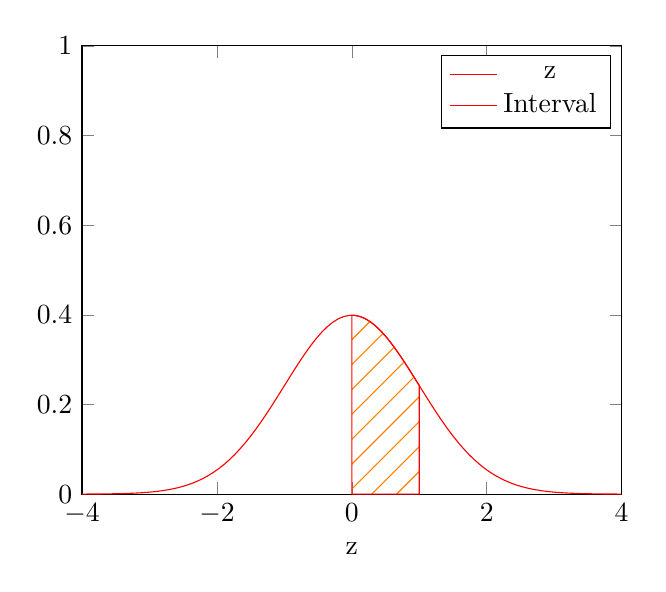
\begin{tikzpicture}
\pgfdeclarepatternformonly{north east lines wide}%
   {\pgfqpoint{-1pt}{-1pt}}%
   {\pgfqpoint{10pt}{10pt}}%
   {\pgfqpoint{9pt}{9pt}}%
   {
     \pgfsetlinewidth{0.4pt}
     \pgfpathmoveto{\pgfqpoint{0pt}{0pt}}
     \pgfpathlineto{\pgfqpoint{9.1pt}{9.1pt}}
     \pgfusepath{stroke}
    }

    \begin{axis}[xmin=-4,xmax=4,xlabel={z},ymin=0,ymax=1] 
    \addplot[color=red,domain=-4:4,samples=100] {1/sqrt(2*pi)*exp(-x^2/2)};
    \addlegendentry{z}
    \addplot+[mark=none,domain=0:1,samples=100,%
              pattern=north east lines wide,%
              pattern color=red!50!yellow]%
              {1/sqrt(2*pi)*exp(-x^2/2)}
              \closedcycle;
    \addlegendentry{Interval}
    \end{axis}
\end{tikzpicture}
\end{document}
